\documentclass{article}
\usepackage[utf8]{inputenc}

\usepackage[left=2cm,right=2cm,top=2cm,bottom=2cm]{geometry} 
\author{Evelyn Lorena Dubón Sicán , 20181014, dubon181014@unis.edu.gt} 
\title{Hoja de trabajo No.1} 
\date{25 de julio del 2018} 
\usepackage{natbib}
\usepackage{graphicx}
% Margins 
\topmargin= -0.45in 
\evensidemargin=0in
\oddsidemargin=0in
\textwidth=6.5in
\textheight=9.0in
\headsep=0.25in
\begin{document}

\maketitle

\section{Pregunta 1}
\begin{itemize}
    \item El conjunto de nodos : \[ 
\left \{
  1, 2, 3, 4, 5, 6, 7
\right \}
\]
    \item  El conjunto de vertices del grafo:\[ 
\Bigg \{
  \begin{tabular}{cccccc}
\big\langle1,2\big\rangle &,\big\langle1,3\big\rangle &,\big\langle1,4\big\rangle &, \big\langle1,5\big\rangle &, \big\langle1,6\big\rangle \\
\big\langle2,1\big\rangle &,\big\langle2,3\big\rangle &,\big\langle2,4\big\rangle &, \big\langle2,5\big\rangle &, \big\langle2,6\big\rangle \\
\big\langle3,1\big\rangle &,\big\langle3,2\big\rangle &,\big\langle3,4\big\rangle &, \big\langle3,5\big\rangle &, \big\langle3,6\big\rangle \\
\big\langle4,1\big\rangle &,\big\langle4,2\big\rangle &,\big\langle4,3\big\rangle &, \big\langle4,7\big\rangle &, \big\langle5,1\big\rangle \\
\big\langle5,2\big\rangle &, \big\langle5,3\big\rangle &, \big\langle5,4\big\rangle &, \big\langle5,6\big\rangle &, \big\langle5,7\big\rangle \\
\big\langle6,1\big\rangle &, \big\langle6,2\big\rangle &, \big\langle6,3\big\rangle &, \big\langle6,5\big\rangle &, \big\langle6,7\big\rangle \\
\big\langle7,3\big\rangle &, \big\langle7,4\big\rangle &, \big\langle7,5\big\rangle &, \big\langle7,6\big\rangle
  \end{tabular}
  \Bigg \}
\] 
\center 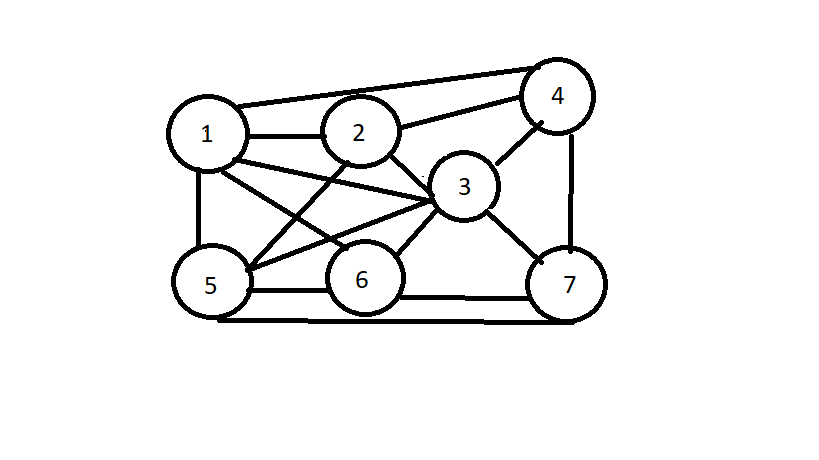
\includegraphics{Grafo.png}    
\end{itemize}
\section{Pregunta 2}
\sum_{i=1}^{n}{i}=\frac{n(n+1)}{2} \par
 Caso Base \par
 n=1\par
\center \sum_{i=1}^{1}{i}=\frac{1(1+1)}{2}\par
\center \sum_{i=1}^{1}{i}=\frac{1(2)}{2}\par
\center \sum_{i=1}^{1}{i}=\frac{2}{2} \par
\center  \sum_{i=1}^{n}{i}={1}\par
\begin{flushleft}
Caso Inductivo \par
n=n\oplus1\par
\end{flushleft}
\center \sum_{i=1}^{n+1}{i}=\frac{n\oplus1((n\oplus1)\oplus1)}{2}
\center \sum_{i=1}^{n+1}{i}=\frac{(n\oplus1)(n\oplus2)}{2}
\center \sum_{i=1}^{n+1}{i}=\frac{n\oplus1}{1}\otimes \frac {n\oplus2}{2}
\center \sum_{i=1}^{n+1}{i}=\frac{n\oplus1}{1}\otimes \frac {n\oplus2}{2}
\center \sum_{i=1}^{n+1}{i}=\frac{n\oplus1}{1}\otimes (\frac {n}{2} \oplus \frac{2}{2})
\center \sum_{i=1}^{n+1}{i}=\frac{n(n\oplus1)}{2}\oplus\frac{(n \oplus 1)}{1}
\center \sum_{i=1}^{n+1}{i}=\frac{n(n\oplus1)\oplus2(n \oplus 1)}{2}
\center \sum_{i=1}^{n+1}{i}=\frac{(n\oplus1)\otimes(n\oplus2)}{2}
\center \sum_{i=1}^{n+1}{i}=\frac{n\oplus1((n\oplus1)\oplus1)}{2}
\begin{flushleft}
\section{Pregunta 3}
\end{flushleft}
\begin{center}
\[

       \sum(n)=1+2+3+4+\ \ldots\ n=
\left\{
     \begin{array}{ll}
 0  & \mbox{si } n = 0 \\
 1 & \mbox{si } n = 1 \\
 \frac{n(n+1)}{2} & \mbox{si } n = s(i) \\

   \end{array}

\end{center}
\section{Pregunta 4}
\end{flushleft}
\begin{center}
 \begin{array}{l l}
b & \mbox{si } a=o \\
a & \mbox{si } b=o \\
\end{array} \par
\begin{center}
Caso base \par
\begin{center}
a =0 \par
\begin{center}
0 \oplus b = b \oplus 0 \par
\begin{center}
b=b \par
\begin{center}
Caso Inductivo \par 
\begin{center}
s(i)\oplus b = b \oplus s(i) \par
\begin{center}
s(i \oplus b) = s(i \oplus b)\par  
\end{center}
\begin{flushleft}
\section{Pregunta 5}
\end{flushleft}
\begin{flushleft}
((n\oplus n)\geq n) = s(0)
\end{flushleft}
\begin{center}
    Caso base \par
\end{center}
\begin{center}
    n=0 \par
\end{center}
\begin{center}
    ((0 \oplus 0) \geq 0) \par
 \end{center}
 \begin{center}
    0\geq 0 \par
    \end{center}
    \begin{center}
    Caso Inductivo \par
    \end{center}
    \begin{center}
    n= s(0) \par
    \end{center}
    \begin{center}
    ((s(0) \oplus s(0)) \geq s(0)) \\
    \end{center}
    \begin{center}
    ((s(s(0 \oplus 0))) \geq s(0))  \\
    \end{center}
    \begin{center}
    ((s(s(0))) \geq s(0))  \\
    \end{center}
    \begin{center}
    (s(s(0)) \ominus s(0) \geq 0) \par\\
    \end{center}
    \begin{center}
    (s(0) \geq 0)
    \end{center}
    (((n \oplus n) \geq n) = s(0)) = s(0)
\endgroup
\end{document}
